\documentclass[serif]{beamer}

\newcommand{\LE}{\emph{Let's Encrypt~}}%
\newcommand{\LEs}{\emph{Let's Encrypt}}%
\usenavigationsymbolstemplate{}
\addtobeamertemplate{navigation symbols}{}{%
    \usebeamerfont{footline}%
    \usebeamercolor[fg]{footline}%
    \hspace{1em}%
    \insertframenumber/\inserttotalframenumber
}


\usepackage{hyperref}

\hypersetup{
    colorlinks,%
    citecolor=red,%\ne
    filecolor=black,%
    linkcolor=blue,%
    urlcolor=red
}

\setbeamerfont{footline}{series=\bfseries, size=\footnotesize}

\title{Anomaly Detection on DNS Auths }
\subtitle{Root DNS, ccTLDs and DNS providers}

\author[\large \textbf{Team  Schnabeltier}

]
{\large \textbf{Team  Schnabeltier}\\
\vspace{0.5cm}
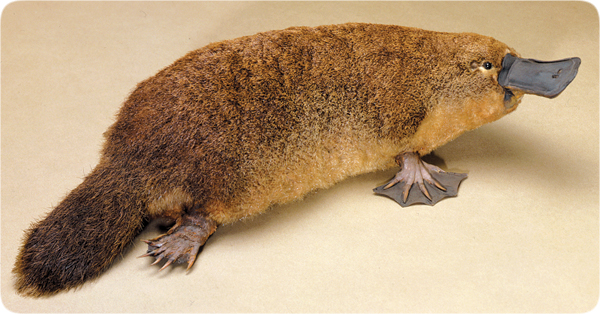
\includegraphics[width=5cm]{fig/Schnabeltier.jpg}
}

\date[IETF98] % (optional)
{RIPE DNS Hackaton 2017\\Amsterdam, The Netherlands\\
2017-04-21}

% \logo{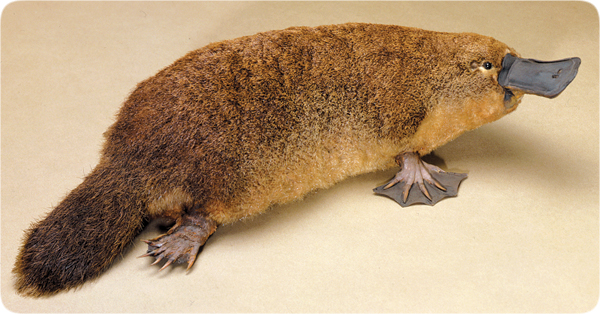
\includegraphics[scale=0.051]{fig/Schnabeltier.jpg}}

\begin{document}
\frame{\titlepage}

\section{At a glance}

\begin{frame}
	\frametitle{Team Members (alphabetically)}
	
	\begin{itemize}
	\item Christian Doerr (TU Delft)
	\item Ella 
	\item Giovane Moura (SIDN Labs)
	\item Jan Harm Kuipers (University of Twente/SIDN Labs)
	\item Moritz M\"uller (SIDN Labs/University of Twente)
	\item Ricardo Schmidt (University of Twente)
	\item Wouter de Vries (University of Twente)
% 	\item 
	\end{itemize}


\end{frame}

\begin{frame}
	\frametitle{Resources}
	
	\begin{itemize}
	  \item GitHub: \url{https://github.com/orgs/ripe-dns-anomaly/}
	  \item Demo: \url{https://ripe-dns-anomaly.github.io}
	\end{itemize}


\end{frame}



\begin{frame}
	\frametitle{Main Problem}
	
	\begin{block}{Auth DNS Anomaly Detection}
	\begin{itemize}
	 \item \textit{How can we use Ripe Atlas data to detect automatically 
failures on Auth DNS (Roots, ccTLDs, etc...)?}
	\end{itemize}

	\end{block}

\end{frame}



\end{document}
